\cleardoublepage



\chapter{Introduction de l'étude}
\label{Introduction de l'étude}

%%%%%%%%%%%%%%%%%%%%%%%%%%%%%%%%%%%%%%%%%%%%%%%%%%%%%%%%%%%%%%%%%%%%%%%%%%%%%%%%%%%%%%%%%%%%%%%%%%%%
%%%%%%%%%%%%%%%%%%%%%%%%%%%%%%%%%%%%%%%%%%%%%%%%%%%%%%%%%%%%%%%%%%%%%%%%%%%%%%%%%%%%%%%%%%%%%%%%%%%%
%%%%%%%%%%%%%%%%%%%%%%%%%%%%%%%%%%%%%%%%%%%%%%%%%%%%%%%%%%%%%%%%%%%%%%%%%%%%%%%%%%%%%%%%%%%%%%%%%%%%
%%%%%%%%%%%%%%%%%%%%%%%%%%%%%%%%%%%%%%%%%%%%%%%%%%%%%%%%%%%%%%%%%%%%%%%%%%%%%%%%%%%%%%%%%%%%%%%%%%%%
%%%%%%%%%%%%%%%%%%%%%%%%%%%%%%%%%%%%%%%%%%%%%%%%%%%%%%%%%%%%%%%%%%%%%%%%%%%%%%%%%%%%%%%%%%%%%%%%%%%%

\section{Besoin de l'utilisateur}

L'envoi de SMS depuis son ordinateur possède plusieurs avantages par rapport à l'envoi depuis un smartphone.
\\


Il est beaucoup plus aisé d'écrire un texte depuis un clavier d'ordinateur, plutôt que sur un écran tactile ou un clavier à très petites touches.
Cela peut aussi aider les personnes ayant des difficultés avec les smartphones, comme par exemple les personnes malvoyantes.
\\


Tout le monde n'a pas accès instantanément à son smartphone lorsque l'on utilise un ordinateur.
Celui-ci peut être dans notre poche, dans un sac, posé sur une table distante, \ldots et l'on aimerait écrire lire ou répondre à des SMS sans avoir à se déplacer tout en gardant les yeux sur l'écran et les mains sur le clavier.
\\





%%%%%%%%%%%%%%%%%%%%%%%%%%%%%%%%%%%%%%%%%%%%%%%%%%%%%%%%%%%%%%%%%%%%%%%%%%%%%%%%%%%%%%%%%%%%%%%%%%%%
%%%%%%%%%%%%%%%%%%%%%%%%%%%%%%%%%%%%%%%%%%%%%%%%%%%%%%%%%%%%%%%%%%%%%%%%%%%%%%%%%%%%%%%%%%%%%%%%%%%%
%%%%%%%%%%%%%%%%%%%%%%%%%%%%%%%%%%%%%%%%%%%%%%%%%%%%%%%%%%%%%%%%%%%%%%%%%%%%%%%%%%%%%%%%%%%%%%%%%%%%
%%%%%%%%%%%%%%%%%%%%%%%%%%%%%%%%%%%%%%%%%%%%%%%%%%%%%%%%%%%%%%%%%%%%%%%%%%%%%%%%%%%%%%%%%%%%%%%%%%%%
%%%%%%%%%%%%%%%%%%%%%%%%%%%%%%%%%%%%%%%%%%%%%%%%%%%%%%%%%%%%%%%%%%%%%%%%%%%%%%%%%%%%%%%%%%%%%%%%%%%%

\section{Solutions existantes}

Les solutions actuellement proposées aux utilisateurs sont très limitées, ce qui explique le fait que très peux d'entre-eux sont utilisées.
\\


Chez certains opérateurs de téléphonie mobile le service SMS peut couter plus de 0,10\texteuro par envoi, et les tarifs des sites indépendants affichent des prix voisins.
Des solutions gratuites existent et permettent des envois gratuits sur internet, mais ceux-ci sont limités à quelques envois ou bien demande une confirmation pour éviter les abus.

Un inconvénient remarquable parmi toutes les solutions existantes est l'absence de gestion des contacts.
En effet l'utilisateur est obligé de spécifier "à la main" le numéro de téléphone du destinataire.
Cela est fastidieux car il faut soit connaitre le numéro par cœur, soit accéder à son carnet d'adresse qui se trouve souvent sur son smartphone.

La dernière remarque que nous pouvons faire sur les solutions existantes est le fait que la réception des SMS n'est gérée.
Cela peut s'expliquer par le fait que la réception de SMS nécessite une mémorisation du message (dans le logiciel ou sur le serveur web), contrairement à l'envoi.
\\





%%%%%%%%%%%%%%%%%%%%%%%%%%%%%%%%%%%%%%%%%%%%%%%%%%%%%%%%%%%%%%%%%%%%%%%%%%%%%%%%%%%%%%%%%%%%%%%%%%%%
%%%%%%%%%%%%%%%%%%%%%%%%%%%%%%%%%%%%%%%%%%%%%%%%%%%%%%%%%%%%%%%%%%%%%%%%%%%%%%%%%%%%%%%%%%%%%%%%%%%%
%%%%%%%%%%%%%%%%%%%%%%%%%%%%%%%%%%%%%%%%%%%%%%%%%%%%%%%%%%%%%%%%%%%%%%%%%%%%%%%%%%%%%%%%%%%%%%%%%%%%
%%%%%%%%%%%%%%%%%%%%%%%%%%%%%%%%%%%%%%%%%%%%%%%%%%%%%%%%%%%%%%%%%%%%%%%%%%%%%%%%%%%%%%%%%%%%%%%%%%%%
%%%%%%%%%%%%%%%%%%%%%%%%%%%%%%%%%%%%%%%%%%%%%%%%%%%%%%%%%%%%%%%%%%%%%%%%%%%%%%%%%%%%%%%%%%%%%%%%%%%%
%%%%%%%%%%%%%%%%%%%%%%%%%%%%%%%%%%%%%%%%%%%%%%%%%%%%%%%%%%%%%%%%%%%%%%%%%%%%%%%%%%%%%%%%%%%%%%%%%%%%

\section{Solution envisagée}

Pour établir notre cahier des charges nous avons étudié les solutions existantes puis étudiés leurs principaux défauts pour produite une solution optimale pour l'utilisateur.
\\


Sachant que la quasi totalité des forfaits mobiles autorisent un nombre illimité d'envois de SMS, nous voulons donc que les utilisateurs utilisent leur propre forfait mobile pour effectuer les envois et réceptions de SMS depuis l'ordinateur, en utilisant un protocole de communication qui transférerait les données.

Nous avons décidé d'intégrer la réception des SMS dans notre solution.
Cette fonctionnalité devra se faire de manière sécurisée et confidentielle.

Enfin nous avons voulu proposer une gestion simple des contacts de l'utilisateur lui permettant de ne pas à avoir à entrer le numéro de téléphone.
De même que pour la réception des SMS, les contacts devront être sûre.
\\


Le schéma ci-dessous représente le fonctionnement général de la solution.
Les flèches vertes indiquent le cheminement du message lors de l'envoi, et les flèches bleues indiquent le cheminement du message lors de la réception.

\begin{figure}[!h]
	\center
	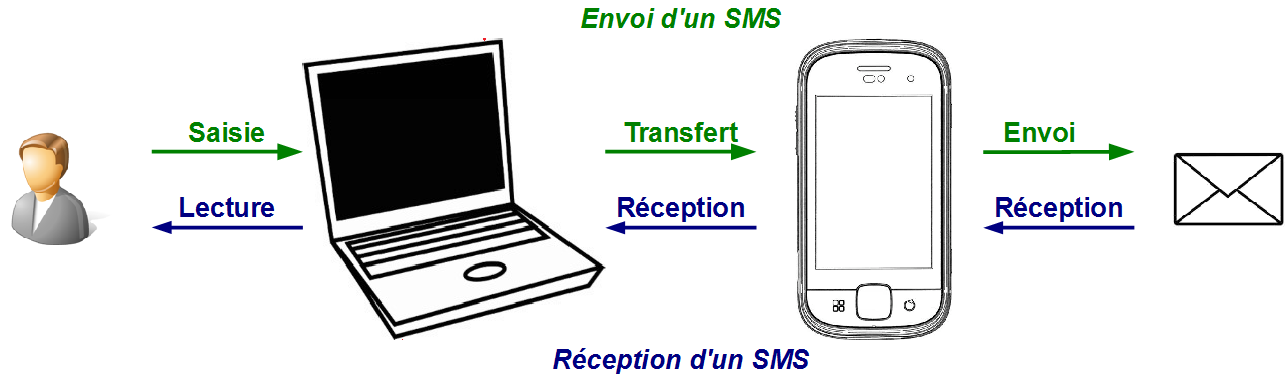
\includegraphics[width=0.9\textwidth]{img/schemaFonctionnement_general.png}
	\caption{Fonctionnement général}
	\label{schemaFonctionnement_general}
\end{figure}

